\vsssub
\subsubsection{~$S_{ref}$: Energy reflection at shorelines and icebergs} \label{sec:REF1}
\vsssub

\opthead{REF1}{\ws}{F. Ardhuin}

\noindent 
Reflections by shorelines and icebergs is activated by using the {\code REF1}
switch and setting namelists parameters {\code REFCOAST}, {\code REFSUBGRID}
or {\code REFBERG} (in namelist {\F REF1}) to non-zero values that are the
target reflection coefficients $R_0^2$ for the wave energy.  If the {\code
IG1} switch is also used, then the energy source at the shoreline also
includes free infragravity waves in both ingoing and outgoing directions.
That particular source is described in section
\ref{sec:IG1}.

From these values $R_0^2$ may be varied with wave height and period following
a Miche-type parameter: this is activated by setting {\code REFFREQ} to a
non-zero value, and is based on the field measurements of \cite{art:EHG94}.
These coefficients can also be made to vary spatially, by setting {\code
REFMAP} to a non-zero value. In that case ww3\_grid will expect to find a
extra line after the reading of the water depths and obstructions in
ww3\_grid.inp, which will define the map of shoreline slopes. The values in this map 
are multiplied by the value {\code REFMAP}.

Wave reflection at the shoreline varies from a fraction of a percent to about
50\% of the incoming wave energy, and may have important consequences for the
directional wave spectrum, and the wave climate in otherwise sheltered
locations \citep{pro:ORe99}. Wave reflection is also extremely important for
the generation of seismic noise by ocean waves.

Because reflection involve wave trains with different directions, in a model
like \ws, their interaction can only be represented through a source term in
the right hand side. Nevertheless, this is physically linked to propagation.

In practice, for the regular and curvilinear grids, the reflection source term
puts into the reflected wave directions the proper amount of energy that will
be taken away by propagation at the next time step. When neglecting the
cross-shore current, this is

\begin{equation} 
\cS_{ref}(k,\theta) = 
\int R^2(k,\theta,\theta') \frac{C_g(k)}{\Delta A} \left[\cos (\theta-\theta_q) \Delta q + \sin (\theta-\theta_p)  \Delta p \right] N(k,\theta') \mathrm{d} \theta' \; ,
\end{equation}

\noindent
where $R^2$ is an energy reflection coefficient, and $\Delta p$ and $\Delta q$
are the grid spacing along the two axes of the grid, and $\Delta A$ is the
cell area. The definition of the shoreline direction from the land/sea mask is
explained in \cite{art:Aea11}. This has not been tested for the SMC grids, and
it is not expected to work for that type of grid.

In the case of unstructured grids, the spectral density of outgoing directions
on the boundary is directly set to the expected reflected value and the
boundary condition is handled specifically by the the numerical schemes.


The reflection coefficient $R^2$ is taken to be non-zero only for the
directions for which $\cos(\theta-\theta')<0$, and its magnitude is the
product of a reflection coefficient $R_0^2(k)$, integrated over the scattered
directions $\theta$, and a directional distribution $R_2(\theta,\theta')$
around the specular direction $\theta_s$,

\begin{equation} 
R^2(k,\theta,\theta')  =  R_0^2(k) R_2(\theta,\theta') \:\:\: .
\end{equation}

\noindent
This directional distribution takes three forms: 
\begin{itemize}

\item isotropic in all directions opposite to the incoming direction: this is
      for sub-grid islands and icebergs or sharp shoreline angles, 

\item proportional to $\cos(\theta-\theta_s)^2$ for moderate shoreline angles,

\item proportional to $\cos(\theta-\theta_s)^n$ for small shoreline angles
      (nearly straight shoreline). Where $n=4$ by default and can be changed
      to any value using the {\code REFCOSP\_STRAIGHT} namelist parameter in
      the {\F REF1} namelist.

\end{itemize}

\noindent
That parameterization is described in detail by \cite{art:AR12}.

In the case of icebergs and sub-grid islands, the reflected energy is
redistributed evenly in all directions within 90$\degree$ of the direction
opposite to the incoming waves.  For resolved lands, a mean direction
perpendicular to shore $\theta_n$ was defined from the land or sea status of
the 8 grid points surrounding the local point (Fig. \ref{fig:refl}).

For each model grid point adjacent to land, the analysis of the land-sea
geometry gives one value of $\theta_n$ among 16 possible directions. Together
with any incoming wave direction $\theta_i$ this defines a specular reflection
direction $\theta_r=2 \theta_n - \theta_i + \pi$.  For each spectral component
of direction $\theta_i$ going towards the coast (i.e. such that
$\cos(\theta_i-\theta_n) >0$), the total reflection is $R^2$ times the
incoming energy. This reflected energy $R^2 E(f) M(f,\theta_i)$ is
redistributed over directions around the specular reflection direction
$\theta_r$, with a broad distribution taken proportional to
$\cos^n(\theta-\theta_r)$, where the power $n$ is a function of the local
shoreline geometry.

\begin{figure} \begin{center}
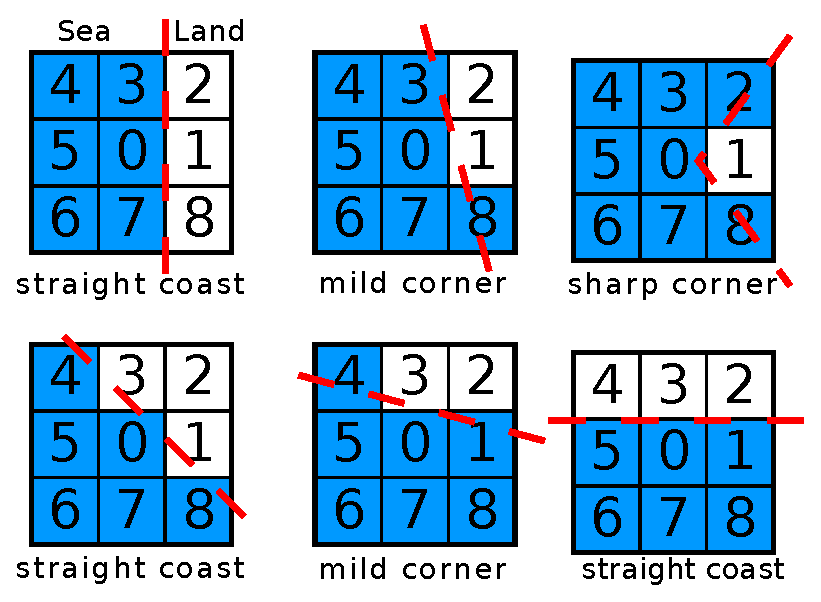
\epsfig{file=./num/coast_reflection.eps,angle=0,width=3in}
\caption{Examples of determination of the shoreline orientation and geometry
  using the land/sea mask. For any sea point (number 0) which is the ocean
  (in blue) and has at least one neighbor in land (in white) the eight
  neighbors, numbered from 1 to 8 are used to define the shoreline geometry.
  For `mild' corners and straight coasts, the estimated shoreline orientation
  (dashed line) is used to compute the directional distribution of the
  reflected wave energy.  }
\label{fig:refl} \botline
\end{center}
\end{figure}

For this purpose we distinguish three different shoreline geometries relative
to the local point as illustrated by Fig. \ref{fig:refl}: we set $n=2$ for a
straight coast (three connected land points among the neighbors), $n=1$ for a
mild corner (two land points among the neighbors), and $n=0$ at a sharp corner
(only one land point, among the 4 closest neighbors) which corresponds to the
same treatment done for sub-grid islands and icebergs. Changing these values
of $n$ in the range $0$ to $2$ has little effect on our results.  $n=1$
corresponds to a Lambertian surface approximation, which is used for
electromagnetic wave scattering from rough surfaces. A pure specular
reflection would be obtained with $n$ infinite.  A more rigorous treatment
should use the distribution of the shoreline orientation at at the scale of
the ocean wavelength, namely of the order of 100~m.
